% --------------------------------------------------------------
% This is all preamble stuff that you don't have to worry about.
% Head down to where it says "Start here"
% --------------------------------------------------------------

\documentclass[10pt]{beamer}

% \usepackage[margin=1in]{geometry}
\usepackage{amsmath,amsthm,amssymb}
\usepackage{enumitem}
\usepackage{tikz}
\usepackage{wrapfig}
\usepackage{cjhebrew}
% \usepackage[shortlabels]{enumerate}

\usepackage[utf8]{inputenc}
\usepackage[english]{babel}

\usetikzlibrary{calc}
\usetikzlibrary{arrows.meta}
\usetikzlibrary{arrows}

\newcommand{\NN}{\mathbb{N}}
\newcommand{\ZZ}{\mathbb{Z}}
\newcommand{\QQ}{\mathbb{Q}}
\newcommand{\RR}{\mathbb{R}}
\newcommand{\CC}{\mathbb{C}}

\newcommand{\CVect}{\CC\operatorname{-Vect}}
\newcommand{\card}{\operatorname{card}}
\newcommand{\diam}{\operatorname{diam}}
\newcommand{\id}{\operatorname{id}}
\newcommand{\interior}{\operatorname{int}}
\newcommand{\lcm}{\operatorname{lcm}}
\newcommand{\Lip}{\operatorname{Lip}}
\newcommand{\norm}[1]{\left\lVert#1\right\rVert}

\newcommand{\Spec}{\operatorname{Spec}}

\renewcommand{\Re}{\operatorname{Re}}
\renewcommand{\Im}{\operatorname{Im}}

\newtheorem{conjecture}{Conjecture}
\newtheorem{question}{Question}

\usepackage[backend=bibtex,style=alphabetic,maxcitenames=50,maxnames=50]{biblatex}
\addbibresource{ultrapowerful.bib}
\renewbibmacro{in:}{}
\DeclareFieldFormat{pages}{#1}

\usetheme{AnnArbor}
\usecolortheme{dove}

\begin{document}
\title{UltraPOWER!}
\author{Aidan Backus}
% --------------------------------------------------------------
%                         Start here
% --------------------------------------------------------------
\begin{frame}
    \titlepage
\end{frame}

\begin{frame}{Philosophical remarks}
    In this talk: We discuss the proof strategy of passing to a nonstandard model.

    The idea is if you study a mathematical theory $T$, there is a ``standard model" $M$ of $T$, which is the object you're actually studying.

    \pause

\begin{example}
    The standard model of algebraic number theory is $\overline \QQ$, the standard model of analysis is $\RR$, and the standard model of arithmetic is $\NN$.
\end{example}

    \pause

    In addition to the standard model $M$, there exist nonstandard models $*M$, which satisfy the same basic properties that $T$ imposes, but are equipped with an embedding $j: M \to *M$ which witnesses that $*M$ is much larger than $M$. The point is that because $*M$ is so big, it's easier to prove things in $*M$ than it is in $M$.

\pause

    Luckily, even though our proofs are analytic (in the sense that they depend on a choice of model), the conclusions are still model-independent thanks to $j$.
\end{frame}

\begin{frame}{Philosophical remarks}
    In this talk, we'll build two nonstandard models:

\pause

\begin{example}
    We'll build a nonstandard model $*\overline \QQ$ of algebraic number theory which is uncountable, allowing us to prove the Nullstellensatz.
\end{example}

\pause

\begin{example}
    We'll build a nonstandard model $*\CC$ of complex analysis, which contains a nonstandard model $*\RR$ of analysis and a nonstandard model of $*\NN$ of arithmetic. In this model, there exists $n \in *\NN$ such that if a polynomial $f$ has degree $n$, then $f$ has infinitely many zeroes in $*\CC$. In this model, we will be able to prove Sendov's conjecture in high degree.
\end{example}

\pause

    The embedding $j: M \to *M$ isn't an isomorphism, but it preserves the theory $T$, so we can transfer these proofs back down into the standard model $M$.
\end{frame}

\begin{frame}{Łoś' theorem}
    Fix a first-order language $\mathcal L$. (So $\mathcal L$-formulae can refer to objects in a $\mathcal L$-structure \textbf{but not sets of objects}).

\pause

\begin{example}
    The language $\mathcal L$ of ordered rings consists of logical symbols as well as $+,\cdot,0,1,\leq$. A typical $\mathcal L$-structure is $\mathbb Q$ and a typical $\mathcal L$-formula $\varphi$ is
    $$\forall a \forall b \forall c(\exists x(ax^2 + bx + c = 0) \leftrightarrow (4ac \leq b^2)),$$
    thus $\QQ \not \models \varphi$ but $\RR \models \varphi$.
\end{example}

\pause

\begin{definition}
    Let $M, N$ be $\mathcal L$-structures.
    A map $j: M \to N$ is an \emph{elementary embedding} if for every $x \in M^n$ and $\mathcal L$-formula $\varphi$ with $n$ free variables,
    $$M \models \varphi(x_1, \dots, x_n)\text{ iff } N \models \varphi(j(x_1), \dots, j(x_n)).$$
    In that case we call $N$ an \emph{elementary extension} of $M$.
\end{definition}
\end{frame}

\begin{frame}{Łoś' theorem}
    For now when I say ``measure" I mean finitely additive. (Why? Stay tuned.)

\begin{definition}
    A measure $\mu$ is \emph{boolean-valued} if for every measurable set $E$, $\mu(E) \in \{0, 1\}$.
\end{definition}

\pause

\begin{theorem}[boolean prime ideal theorem]
    There is a nonatomic, boolean-valued measure on the power set of $\NN$.
\end{theorem}

\pause

\begin{definition}
    Let $X$ be a set, $\mu$ a boolean-valued measure on the power set of $X$. The \emph{ultrafilter} $U$ on $X$ associated to $\mu$ is $U = \{A \subseteq X: \mu(A) = 1\}$.
\end{definition}

\pause

  The boolean prime ideal theorem follows immediately from Zorn's lemma. By the boolean prime ideal theorem, there is a nonatomic ultrafilter on $\NN$.
\end{frame}

\begin{frame}{Łoś' theorem}
\begin{definition}
    Let $M$ be an $\mathcal L$-structure and $U$ an ultrafilter on $M$.
    Let $M^\NN$ be the space of sequences in $M$. We get an equivalence relation on $M^\NN$ by setting $x \sim y$ if $\{n \in \NN: x_n = y_n\} \in U$.

\pause

    The \emph{ultrapower} $M[U]$ is the set of residue classes.
\end{definition}

\pause

    Thus $M[U]$ is the space of maps $\NN \to M$ modulo being equal $U$-almost everywhere. Therefore all operations on $M$ drop to operations on $M[U]$, just as operations on $\CC$ drop to operations on $L^2(X \to \CC)$. So $M[U]$ is a $\mathcal L$-structure.

\pause

    \begin{theorem}[Łoś]
        Let $M$ be a structure, $U$ an ultrafilter, and define a map $j: M \to M[U]$ by $j(x) = [x, x, \dots]$.
        Then $j$ is an elementary embedding.
    \end{theorem}

\pause

    The proof is by induction on complexity. Use the axiom of choice to choose a representative for the $\exists$ case.
\end{frame}

\begin{frame}{Łoś' theorem}

\begin{definition}
    A \emph{measurable cardinal} $\kappa$ is the cardinality of a set $A$ such that there is a \textbf{countably additive} nonatomic ultrafilter on $A$.
\end{definition}

\pause

\begin{theorem}[Scott, Ulam, and Keisler]
    If $\kappa$ is measurable, then there is an elementary embedding $j$ of the class of all sets such that $j(\kappa) > \kappa$.
    In particular, the set of Grothendieck universes of rank $\leq \kappa$ has cardinality $\kappa$.
\end{theorem}

\pause

\begin{center}
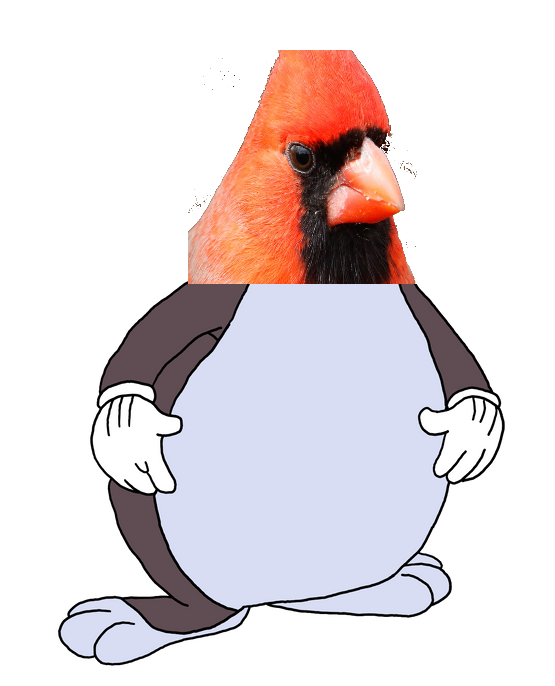
\includegraphics[scale=0.18]{chungus_cardinal}
\end{center}
\end{frame}

\begin{frame}{The Nullstellensatz}
    \begin{theorem}[The Nullstellensatz]
    Let $I$ be an ideal of polynomials over an algebraically closed field $k$ and $V$ be the variety determined by $I$. Then $\sqrt I$ is the ideal of polynomials that vanish on $V$.
    \end{theorem}

\pause

    Suppose that $k$ is uncountable. Then by an easy exercise in Eisenbud, the Nullstellensatz holds. (The point is that a certain field $F$ has countable dimension over $k$, so if $F$ is a proper extension of $k$, then $F$ is countable.)

\pause

    The language of rings doesn't know how to talk about ideals of polynomials, so we first expand it.
    For simplicity we assume $k$ is an extension of $\QQ$ but this assumption can be easily dropped by using a more complicated coding scheme.
\end{frame}

\begin{frame}{The Nullstellensatz}
Let us call $a \in k^{(1+n)N}$ a \emph{valid code} if the last $nN$ entries in $a$ are in $\NN$, in which case we let
$$F(a)(x) = \sum_{J=1}^N a_J \prod_{j=1}^n x_j^{a_{JN + j - 1}}$$
be the polynomial for which $a$ is a \emph{code}.
\pause
Now we expand the language of rings to a language $\mathcal L$ which contains $\ell$-ary predicates $P_\ell,Q_\ell$ and $\ell+n$-ary operations $R_\ell$.
    We interpret $P_\ell(a)$ to mean that $a$ is a valid code, $Q_\ell(a)$ to mean that $a$ is a valid code and $F(a) \in I$, and $R_\ell(a, x)$ to mean $F(a)(x)$.
\pause

    Let $\mathbf{Nullstell}_{\ell,m,n}(a)$ be the $\mathcal L$-formula
\begin{align*}
P_\ell(a) &\to (\exists b (Q_m(b) \wedge \forall x(R_\ell(a, x)^n = R_m(b, x))) \\
&\qquad \leftrightarrow \forall x((\forall b(Q_m(b) \to (R_m(b, x) = 0)) \to (R_\ell(a, x) = 0))).
\end{align*}
    % That is, for every $a \in k^\ell$, $\mathbf{Nullstell}_{\ell,m,n}(a)$ holds iff $a$ is invalid or there is a polynomial $g \in I$ whose code has length at most $m$ such that $g^n = F(a)$ iff for every $x \in V$, $F(a)(x) = 0$.
    The Nullstellensatz holds in $k$ iff for every $\ell \in \NN$ and $a \in k^\ell$, there are $n, M \in \NN$ such that if $m > M$, $k \models \mathbf{Nullstell}_{\ell,m,n}(a)$.
\end{frame}

%
%Let $J = \{f: f|V = 0\}$. Then $\sqrt I \subseteq J$. Conversely, let $f \notin \sqrt I$, so we can extend $I$ to $\mathfrak p \in \mathsf{Spec} ~R$ such that $f \notin \mathfrak p$.
%Let $F = (k[x_1, \dots, x_n]/\mathfrak p)[f^{-1}]/\mathfrak m$, where $\mathfrak m$ is maximal. Let $\alpha \in F$. Since $\dim_k F$ is countable, the uncountable set $\{(\alpha - c)^{-1}: c \in k\}$ is linearly dependent, so there is a nontrivial algebraic relation $\sum_j a_j(\alpha - c_j)^{-1} = 0$ over $k$. Therefore $\alpha \in k$, so $F = k$. Therefore we have a sequence of maps
%$$k[x_1, \dots, x_n] \to \frac{k[x_1, \dots, x_n]}{\mathfrak p} \to R \to k.$$
%Let $y_i$ be the image of $x_i$ under the sequence.
%Then $y \in V$ (since the sequence included quotienting by $I$), and $f(y) \neq 0$ (since the sequence included localizing at $f$), so $f \notin J$.

\begin{frame}{The Nullstellensatz}
Now let $j: k \to k[U]$ be an ultrapower embedding. \pause
If $k[U]$ is uncountable, then for every $a \in k^\ell$, there are $n, M \in \NN$ such that if $m > M$,
$$k[U] \models \mathbf{Nullstell}_{\ell,m,n}(j(a)),$$
so by Łoś' theorem, $k \models \mathbf{Nullstell}_{\ell,m,n}(a)$.
Therefore $k$ satisfies the Nullstellensatz.

\pause

It remains to show that $k[U]$ is uncountable. Suppose $A = \{[(x_n^m)_n]: m \in \NN\}$ is a countable subset of $k[U]$.
Since $k$ is infinite, there is a total order $<$ without endpoints on $k$.
Choose $y_n > \max(x_n^1, \dots, x_n^n)$.
Then if $y_n = x_n^m$, $n < m$, so $\{n: y_n = x_n^m\}$ is finite. Therefore for every $m$, $[y] \neq [x^m]$, so $A \neq k[U]$. \pause This completes the proof of the Nullstellensatz.
\end{frame}

\begin{frame}{Sendov's conjecture}
\begin{theorem}[Tao 2020 -- Sendov's conjecture in high degree]
    Let $f: \CC \to \CC$ be a polynomial with all zeroes in $\overline{D(0, 1)}$ and let $a$ be a zero of $f$.
    If the degree of $f$ is large enough, then $f$ has a critical point in $\overline{D(a, 1)}$.
\end{theorem}

\pause

    Reasoning in the contrapositive, it suffices to show that if there is an increasing sequence of natural numbers $n_j$ and polynomials $p_j$ such that the degree of $p_j$ is $n_j$ and $p_j$ is a counterexample, then Jeremy Kahn is from the planet Jupiter.

\pause

\begin{center}
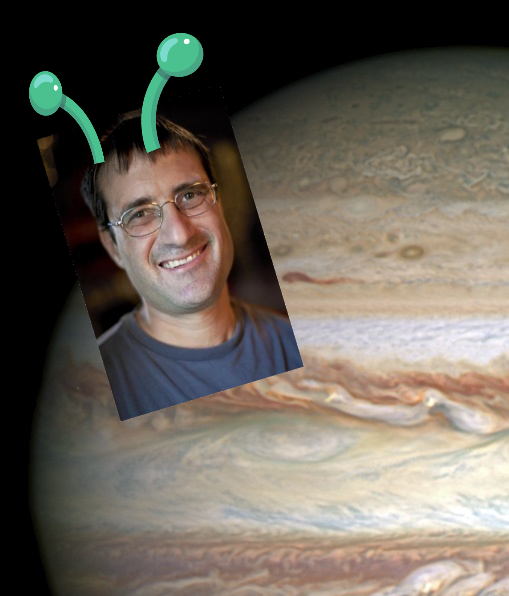
\includegraphics[scale=0.2]{kahn_jupiter}
\end{center}
\end{frame}

\begin{frame}{Sendov's conjecture}
    Let $*\NN = \NN[U]$. We say $*n \in *\NN$ is nonstandard if $*n > j(n)$ for every $n \in \NN$.
    We will actually work with $*\CC = \CC[U]$, which contains copies of $*\RR = \RR[U]$ and $*\NN$.
    (One can construct this by taking a suitable ultrapower of $\CC[x]$ in the language of rings equipped with predicates for $\in \RR$, $\in \NN$, $\leq$, $|\cdot|$, and degree). \pause
    Henceforth we will suppress the stars and always work in this nonstandard model of complex analysis.
    Since there are nonstandard naturals $n$ in this nonstandard model, there are also infinitesimals $1/n$. \pause
    A corollary of Łoś' theorem is:
\begin{theorem}[underspill]
    Let $\varphi$ be a first-order predicate. Suppose that for every nonstandard natural $n$, $\NN \models \varphi(n)$. Then there is an increasing sequence of standard naturals $n_j$ such that $\NN \models \varphi(n_j)$.
\end{theorem}
    Underspill allows us to replace the sequence of polynomials $p_j$ with just a single polynomial $p$ of \emph{nonstandard} degree.
\end{frame}

\begin{frame}{Sendov's conjecture}{Reduction to infinitesimal error}

\begin{wrapfigure}{r}{0cm}

\includegraphics[scale=0.12]{YuriOnIce}
\end{wrapfigure}

Let $n$ be a nonstandard natural, $f$ a monic polynomial of degree $n$ which is a counterexample to Sendov's conjecture, witnessed by a zero $a \in [0, 1]$ such that \pause
\begin{itemize}
\item (\emph{Case Zero}) either $a \log n$ is infinitesimal, \pause
\item (\emph{Case One}) or there is a standard $\varepsilon > 0$ and an infinitesimal $\kappa > 0$ such that $1 - a \in [\varepsilon^n, \kappa]$.
\end{itemize} \pause
It suffices to prove that under these assumptions, Yuri Sulyma is the protagonist of an anime.

\pause

Indeed, if that is true, then by previous work on Sendov's conjecture, ANY nonstandard counterexample will give a contradiction, so underspill completes the proof of Sendov's conjecture in high degree.
\end{frame}

\begin{frame}{Sendov's conjecture}
\begin{lemma}[distributions of random zeroes]
    Fix a random zero $\lambda$ and a random critical point $\zeta$ of $f$, and let $\lambda^{(\infty)}$, $\zeta^{(\infty)}$ be their standard parts.

\pause

    In Case Zero, $\lambda^{(\infty)}$ and $\zeta^{(\infty)}$ are identically distributed and for every compact $K$ which does not intersect $\{e^{i\theta}: \theta \in [\pi/2, 3\pi/2]\}$,
    $$\mathbf P(\lambda \in K) = O(a + n^{-1/3} \log n)$$
    in the sense that $(a + n^{-1/3} \log n)^{-1} \mathbf P(\lambda \in K)$ is finite.

\pause

    In Case One, $\lambda^{(\infty)}$ is uniformly distributed on $\partial D(0, 1)$ and $\zeta^{(\infty)} = 0$ almost surely. Moreover,
    $$\mathbf E \log |\lambda|^{-1}, ~\mathbf E \log |\zeta - a| = O(n^{-1}).$$
\end{lemma}

\pause

This lemma makes no sense if $f$ has standard degree. The idea behind the proof is that a Brownian motion that begins at $\lambda^{(\infty)}$ or at $\zeta^{(\infty)}$ ``looks the same" outside $D(0, 1 + \varepsilon)$.
\end{frame}

\begin{frame}{Sendov's conjecture}{Case Zero}
    Suppose that $a \log n$ is infinitesimal. \pause Let $s(z) = \mathbf E(z - \lambda^{(\infty)})^{-1}$; by the previous lemma, there is almost surely $\theta \in [\pi/2,3\pi/2]$ such that $\lambda^{(\infty)} = e^{i\theta}$, so $s$ is holomorphic on $D(0, 1)$. \pause
    Moreover, there is an annulus $A \subset D(0, 1/2)$ on which $|s| \sim 1$ uniformly, so let $\gamma$ be a loop in $A$. \pause
    If
    $$m = \frac{1}{2\pi i}\int_\gamma \frac{s'(z)}{s(z)} ~dz,$$
    then by the argument principle $m \geq 0$ is the number of zeroes of $s$ in a neighborhood of $0$. \pause
    On the other hand,
    $$\left|\frac{f'}{nf} - s\right|$$
    is infinitesimal in a suitable function space, \pause so by the argument principle, $m$ is the number of zeroes-minus-poles of $f'/f$ near $0$. \pause
    (The tricky bit is justifying this step!) \pause
    But since we are in Case Zero, there is a pole and no zeroes of $f'/f$ near $0$, so $m \leq -1$.
\end{frame}

\begin{frame}{Sendov's conjecture}{Case One}
    In Case One, $\zeta$ is infinitesimal in probability and the standard part of $a$ is $1$. \pause
    Since $\lambda^{(\infty)}$ is uniformly distributed on $\partial D(0, 1)$, $f$ sort of looks like $z^n - 1$.

\pause

    There are critical points of $z^n - 1$ on the arc $\gamma = \partial D(1, 1) \cap \overline{D(0, 1)}$, which are ``almost-counterexamples" to Sendov's conjecture. \pause
    In the general case, there is a compact set $S$, consisting of $\gamma$ and countably many other points, such that $||d(\zeta, S)||_{L^\infty}$ is infinitesimal. \pause
    If
    $$U(z) = \mathbf E \log |z - \zeta|^{-1}$$
    then every zero of $f$ is either ``close to $S$" or ``close to the level set $U = -n^{-1}\log |f(0)|$".
    This gives us precise control on the distributions of $\lambda$ and $\zeta$.

\pause

    After a long computation using underspill and estimates on the variance of $\zeta$, we conclude that $1 - \kappa^n \geq a > 1 - \kappa^n$, a contradiction.
\end{frame}

\begin{frame}{Thanks for coming!!}
    Where I learned all this:

    Ted Slaman, Hugh Woodin, Java Villano, and Matt Park: ``Logic: The UC Berkeley Course"

    Terry Tao: ``Ultrafilters, nonstandard analysis, and epsilon management" (for nonstandard methods in analysis)

    Terry Tao: ``Sendov's conjecture for sufficiently high degree polynomials"

    Peter Koellner and Evan Chen: ``Set Theory"

    Algebraic geometers may also enjoy Tao's essay on ``Ultralimit analysis and quantitative algebraic geometry."

    QUESTIONS?
\end{frame}


\end{document}
